\documentclass[a4paper,fontsize=10pt,twoside,DIV15,BCOR12mm,headinclude=true,footinclude=false,pagesize,bibtotoc]{scrbook}


\usepackage[utf8]{inputenc}
\usepackage[T1]{fontenc}

\usepackage{pslatex} % -- times instead of computer modern
\usepackage[scaled=.84]{beramono} % a sane monospace font
\usepackage{microtype}

\usepackage{url}
\usepackage{booktabs}
\usepackage{graphicx}
\usepackage{textcomp}
\usepackage{xspace}
\usepackage[usenames,dvipsnames,table]{xcolor}
\usepackage{colortbl}
\usepackage{multicol}
\usepackage{rotating}
\usepackage{subfig}
\usepackage{ulem}
\usepackage{enumerate}
\usepackage{fancyvrb}
\usepackage{framed}

% Doxygen includes
\usepackage{calc}
\usepackage{../c_doc/latex/doxygen}
\usepackage{makeidx}
\usepackage{multirow}

% avoid clubs and widows
\clubpenalty=10000
\widowpenalty=10000

% tweak float placement
%% \renewcommand{\textfraction}{.15}
\renewcommand{\topfraction}{.75}
%% \renewcommand{\bottomfraction}{.7}
\renewcommand{\floatpagefraction}{.75}
%% \renewcommand{\dbltopfraction}{.66}
%% \renewcommand{\dblfloatpagefraction}{.66}
\setcounter{topnumber}{4}
%% \setcounter{bottomnumber}{4}
%% \setcounter{totalnumber}{16}
%% \setcounter{dbltopnumber}{4}

\newcommand{\code}[1]{{\texttt{#1}}}
\newcommand{\codefoot}[1]{{\textsf{#1}}}
\def\figref#1{Figure~\ref{fig:#1}}

% ulem package, otherwise emphasized text becomes underlined
\normalem


\newcommand{\todo}[1]{{\emph{TODO: #1}}}
%\renewcommand{\todo}[1]{}

%
% generic command to comment something
%
\newcommand{\ncomment}[3]{

\textsf{\textbf{#1}} {\color{#3}#2}}

%
% commentators
%
\newcommand{\wolf}[1]{\ncomment{Wolfgang}{#1}{OliveGreen}}
\newcommand{\martin}[1]{\ncomment{Martin}{#1}{Blue}}
\newcommand{\rasmus}[1]{\ncomment{Rasmus}{#1}{Mahogany}}

% uncomment to get rid of comments
\renewcommand{\wolf}[1]{}
\renewcommand{\martin}[1]{}
\renewcommand{\rasmus}[1]{}

%
% custom colors
%
\definecolor{lightgray}{gray}{0.8}
\definecolor{gray}{gray}{0.5}

\usepackage{listings}

% general style for listings
\lstset{basicstyle=\ttfamily,keywordstyle=\ttfamily,showstringspaces=false,language=C}

\usepackage[endianness=big]{bytefield}

% long immediate in second slot
\newcommand{\lconst}{\texttt{const}_{32}}
% short immediate in ALU instruction
\newcommand{\sconst}{\texttt{Constant}_{12}}
% constant in Rs2 field
\newcommand{\rconst}{\texttt{Constant}_{5}}

% SH: to be used in text mode .. maybe we should change this to math mode?
\newcommand{\XOR}{\textasciicircum\xspace}
\newcommand{\OR}{\textbar\xspace}
\newcommand{\AND}{\&\xspace}
\newcommand{\NOT}{\texttildelow}
\newcommand{\shl}{\textless$\!$\textless\xspace}
\newcommand{\shr}{\textgreater$\!$\textgreater$\!$\textgreater\xspace}
\newcommand{\ashr}{\textgreater$\!$\textgreater\xspace}

\newcommand{\bitsunused}{\rule{\width}{\height}}
\newcommand{\bitssubclass}{\color{lightgray}\rule{\width}{\height}}

\usepackage{mdwlist}
\renewenvironment{description}%
{
\begin{basedescript}{
\desclabelstyle{\nextlinelabel}
\renewcommand{\makelabel}[1]{%
\parbox[b]{\textwidth}{\bfseries##1}%
}%
\desclabelwidth{2em}}}
{
\end{basedescript}
}

%
% allow click-able links
%
\usepackage[open]{bookmark}
\usepackage[all]{hypcap}

%
% hyperref setup (depends on bookmark/hyperref}
%
\hypersetup{
    pdftitle = {Argo programming exercise},
    pdfsubject = {Technical Report},
    colorlinks = {true},
    citecolor = {black},
    filecolor = {black},
    linkcolor = {black},
    urlcolor = {black},
    final
}

%
% document contents
%
\begin{document}

\title{The Argo software perspective}
\subtitle{A programming exercise}

\author{Rasmus Bo S{\o}rensen}

\lowertitleback{Copyright \copyright{} 2015 Technical University of Denmark
  \medskip\\
  \begin{tabular}{lp{.8\textwidth}}
    \raisebox{-12pt}{
\includegraphics[height=18pt]{fig/cc_by_sa}} &
     This work is licensed under a Creative Commons Attribution-ShareAlike
     4.0 International License.
     \url{http://creativecommons.org/licenses/by-sa/4.0/}\\
  \end{tabular}
}

\frontmatter

\maketitle

\chapter{Preface}

This exercise manual is written for the course `02211 Advanced Computer Architecture' at the Techincal University of Denmark,
but is intended as a stand alone document for anybody interrested in learning to program the Argo Network-on-Chip.

This document is subject to continous development along the the platform it describes.
In case you have suggestions for improvement or find that the text is unclear and needs to be elaborated, please write to \href{mailto:rboso@dtu.dk}{rboso@dtu.dk}

The latest version of this document is contained as LaTeX source in the Patmos repository in directory
\code{patmos/doc/noc} and can be built with \code{make}.

\section*{Acknowledgment}

\tableofcontents

%\begingroup
%\let\cleardoublepage\clearpage
%\listoffigures
%\listoftables
%\lstlistoflistings
%\endgroup

\mainmatter

\chapter{Introduction}

In this document we will present the background required to efficiently program the Argo NoC.
The exercieses should give the reader a good understanding of how the Argo NoC can be utilized in a multicore application.
The reader will get experience in how to write a multicore application that uses message passing.
In the exercises we assume that the reader is familiar with the C programming language and multithreaded programming in general.
Furthermore, we assume that the reader has already run a single core application on a Patmos processor in an FPGA. If this is not the case please refer to the \todo{Patmos exercise manual~\cite{}} for a practical introduction to programming the Patmos processor.


Chapter~\ref{chap:arch} presents the achitecture of the Argo Network-on-Chip.
Chapter~\ref{chap:api} describes the programming interface of the multicore platform, including the thread library and the high level message passing.
Chapter~\ref{chap:exercise} contains the practical exercises ment to give the reader a practical introduction to the platform.
Appendix~\ref{apx:run} describes the practical aspects of loading the program into the platform running in an FPGA.
Appendix~\ref{apx:api} contains the Doxygen documentation of the C libraries.


\chapter{The Architecture of Argo}
\label{chap:arch}
The Argo Network-on-Chip (NoC) is a statically scheduled
time division multiplexed (TDM) NoC that supports
direct memory access (DMA) driven write transactions.
The end points of these write transactions are the dual-ported
processor ĺocal communication scratchpad memories (SPM) connected
on one port directly to the processor and on the other port to the 
network interface, containing the DMA controllers.
Figure~\ref{fig:argo-arch} shows the architecture of the Argo NoC.

\begin{figure}
\centering
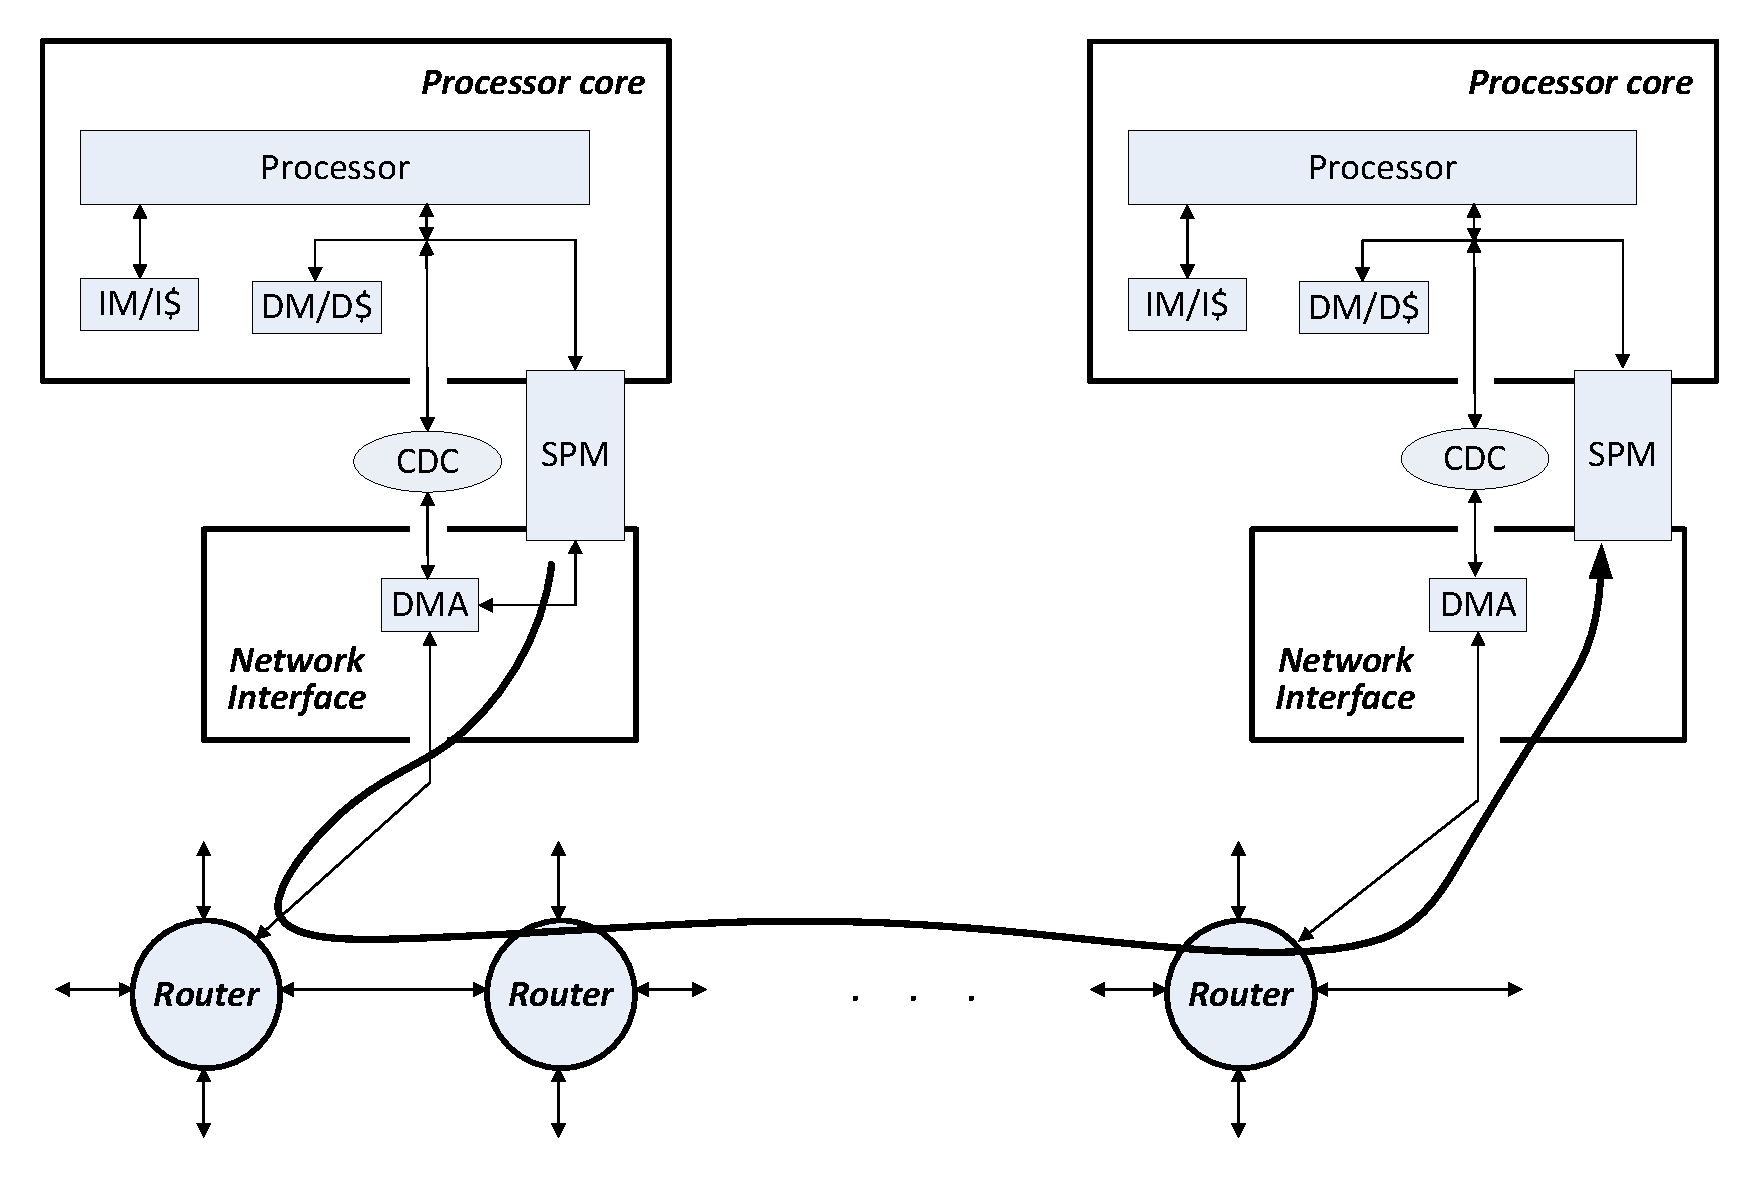
\includegraphics[width=\textwidth]{fig/argo-arch.pdf}
\caption{The Argo architecture from a software perspective. A DMA write transaction moves the specified block of data from the communication SPM of the left processor to the specified location in the communication SPM of the right processor.}
\label{fig:argo-arch}
\end{figure}


% % % % % % % % % % % % % % % % % % % % % % % % % % % % % % % % % % % % % % % %
\chapter{Argo Programming Interface}
\label{chap:api}
In the sections of this chapter we will give an overview of each part of the Argo programming interface.
For detailed documentation refer to Appendix~\ref{ch:dox}, which contains the doxygen documentation of the C libraries.

\section{Corethread Library}
\label{sec:cthread}
When an application is downloaded to the platform, the \code{main()} function is executed on the master core, the master core has the core id 0.
From the \code{main()} function the programmer can execute functions on the slave cores using the functions in the \code{libcorethread} library.
The functions of the \code{libcorethread} library are:
\begin{description}
\item[\code{int corethread\_create( corethread\_t *thread, void(*start\_routine)(void *), void *arg ) )}]

The create function will start the execution of the \code{start\_routine} function on the core specified by \code{thread}, an argument can be given to the started function via the \code{arg} pointer. The start function should only be called by the master core during the initialization phase of the application.

\item[\code{void corethread\_exit( void * retval )}]

The exit function can be called in the \code{start\_routine} functions if they need to return a value to the master core.
The exit function should be called as the last thing before the return statement.

\item[\code{int corethread\_join( corethread\_t thread, void ** retval )}]

The join function will join the program flow of the master core with the program flow of the core specified by \code{thread}, the join function should only be called from the master core. The join function will point the \code{retval} pointer to the return value allocated by the thread on the slave core. Be aware, the return value should not be allocated on the stack of the slave core!

\end{description}


\section{NoC Driver}
The Argo NoC has a very minimalistic interface.
Initialization of the NoC is done before the \code{main()} function starts executing.
To hide the direct interfacing to the hardware, we use the \code{libnoc} that is a driver for the NoC.
If the application requires direct control over data movement through the NoC the three functions presented in the following can be used, otherwise the application should use the message passing library presented in Section~\ref{sec:libmp}.

\begin{description}
\item[\code{int noc\_done( unsigned rcv\_id )}]

The done function is used to tell whether a local DMA transfer has finished.

\item[\code{int noc\_nbsend( unsigned rcv\_id, volatile void \_SPM *dst, volatile void \_SPM *src, size\_t size )}]

The nbsend function is a non-blocking function for sending a block of data at the address \code{dst} of size \code{size} to the core with the core id \code{rcv\_id} and the remote address \code{src}.

\item[\code{void noc\_send( unsigned rcv\_id, volatile void \_SPM *dst, volatile void \_SPM *src, size\_t size )}]

The send function is calling the nbsend in a while loop, until it returns success.
%\item[\code{void noc\_multisend( unsigned cnt, unsigned rcv\_id {[]}, volatile void \_SPM *dst {[]}, volatile void \_SPM *src, size\_t size )}]
%\item[\code{void noc\_multisend\_cs( coreset\_t *receivers, volatile void \_SPM *dst{[]}, unsigned offset, volatile void \_SPM *src, size\_t size )}]
%\item[\code{void noc\_wait\_dma( coreset\_t receivers )}]
\end{description}

\section{Message Passing Library}
\label{sec:libmp}

As the Argo interface (libnoc) does not support receive notification, flow control or double buffering

\begin{description}
\item[\code{int mp\_chan\_init( mpd\_t* mpd\_ptr, coreid\_t sender, coreid\_t receiver, unsigned buf\_size, unsigned num\_buf )}]
\item[\code{int mp\_nbsend( mpd\_t* mpd\_ptr )}]
\item[\code{void mp\_send( mpd\_t* mpd\_ptr )}]
\item[\code{int mp\_nbrecv( mpd\_t* mpd\_ptr )}]
\item[\code{void mp\_recv( mpd\_t* mpd\_ptr )}]
\item[\code{int mp\_nback( mpd\_t* mpd\_ptr )}]
\item[\code{void mp\_ack( mpd\_t* mpd\_ptr )}]
\end{description}

% % % % % % % % % % % % % % % % % % % % % % % % % % % % % % % % % % % % 

\chapter{Exercises}
\label{chap:exercise}
\section{Circulating tokens}
By creating an application that mimics streaming behavior between a number of processors, this exercise will illustrate to the reader how the basics of message passing works on Argo.
In this exercise we will make an application that circulates a number of tokens in a ring of 8 slave processors,
using the default 9 core platform for the Altera DE2-115 board.
The number of tokens should be configurable, but always less than the number for processors.
Each of the processors in the ring shall repeatedly execute the following \ref{list:num1}~steps:

\begin{framed}
\begin{enumerate}
\item Receive a token from the previous processor

\item Turn on the processor LED to indicate that the token is beeing processed

\item Wait for a random amount of time in the interval [100 ms; 1 s]
\label{list:step_rand}
\item Send the token to the next processor, when the send is complete Turn off the processor LED to indicate the the token has been processed

\label{list:num1}\end{enumerate}
\end{framed}

\noindent Looking at the LEDs when the application runs,
the reader should see tokens move from one led to the other.
This behavior should be easy to observe with only few tokens.
This exercise is split into \ref{list:num2}~tasks:
\begin{framed}
\begin{enumerate}
\item Create a function that blinks an LED and create a thread on each slave core that executes the blink function
\item Extend the blink function to turn the LED on and off at random times
\item Extend the blink function to receive a message from the previous core in the ring and send a message to the next core in the ring
\item Change the blink function such that it sends the random seed value along with the token
\label{list:num2}\end{enumerate}
\end{framed}

\noindent In each task you should verify the your program is working as expected by compiling and downloading the program to the platform.

\subsection{Task 1}
In this task you should create a function that blinks the LED and execute the function on the slaves processors.
The frequency of blinking the LED should be in the order of 1~-~10~Hz so that it is visible to the eye.
We suggest to set the frequency of the blinking through a parameter of the blinking function.
Figure~\ref{fig:ctrl_led} shows an example of how to blink an LED.
To turn the LED on and off, write a 1 and 0, respectively to the hardware address of the LED. 

\begin{figure}
\begin{Verbatim}[xleftmargin=1cm,frame=single,framesep=3mm]
// The hardware address of the LED
#define LED (*((volatile _IODEV unsigned *)0xf0000900))
for (;;) {
  for (int i=2000; i!=0; --i)
    for (int j=2000; j!=0; --j)
      // Turn off LED
      LED = 1;

  for (int i=2000; i!=0; --i)
    for (int j=2000; j!=0; --j)
      // Turn off LED
      LED = 0;
}
\end{Verbatim}
\caption{\label{fig:ctrl_led}An example of how to blink an LED}
\end{figure}

To execute the \code{blink()} function on the slave core there is an example of
how to call the \code{corethread\_create()} function in Figure~\ref{fig:corethread}.
Section~\ref{sec:cthread} explains in further detail, how corethreads are started
on slave processors and how a parameter can be passed to the function.

\begin{figure}
\begin{Verbatim}[xleftmargin=1cm,frame=single,framesep=3mm]
void loop(void* arg) {
  int num_tokens = *((int*)arg);
  /*
    Write code in the slave loop
  */
}

int main() {
  corethread_t worker_id = 1; // The core ID
  int parameter = 42;
  corethread_create(&worker_id,&loop,(void*)&parameter);  

  int* res;
  corethread_join(worker_id,&res); // No return value is returned

  return *res;  
}
\end{Verbatim}
\caption{\label{fig:corethread}An example of how to create a corethread.}
\end{figure}

\paragraph*{Expected output}
The 8 LEDs on the board should all blink with the specified frequency.

\subsection{Task 2}
In task 2 you shall extend the blink function from task 1 to turn the LED on and off at random times.
We suggest to use the \code{rand\_r()} function to generate a random number,
\code{rand\_r()} takes a pointer to a seed value in order to generate a random number.
Do not use the \code{rand()} function as it is not thread-safe.
The seed value in each core should be different, otherwise all cores have the
same sequence of psedo-random numbers.

Use the lower bits of the random number to generate a number on the desired range.
The \code{get\_cpu\_usecs()} function returns the value of the microsecond counter as an \code{unsigned long long}. 

\paragraph*{Expected output}
The 8 LEDs should now independently blink with random varying frequencies.

\subsection{Task 3}
In this task you will start sending messages.
Before messages can be sent or received you need to initialize the message passing channels with the \code{mp\_chan\_init()} function.
The use of the message passing function is described in Section~\ref{sec:libmp}.
The initialization of the message passing channels shall be done in the \code{main()} function before the corethreads are started.
If the channels are initialized after the corehtreads are created the behavior of
\code{mp\_send()} and \code{mp\_recv()} is undefined.


\paragraph*{Expected output}
It should now be observable that the tokens move between cores.

\subsection{Task 4}
For the sake of the example, you should now pair a seed value to each tokens.
To send the seed value along with the message, you need to write the seed value into
the \code{write\_buf} before sending the message, and read out the seed value from the \code{read\_buf}
after receiving a message.
Figure~\ref{fig:msg_data} shows an example of how message data can be read and written.

\begin{figure}
\begin{Verbatim}[xleftmargin=1cm,frame=single,framesep=3mm]
// Reading a value from the channel read buffer
seed = *((volatile unsigned int _SPM *)(&chan.read_buf));

// Writing a value to the channel write buffer
*(volatile unsigned int _SPM *)(&chan.write_buf) = seed; 
\end{Verbatim}
\caption{\label{fig:msg_data}An example of how to read and write message data}
\end{figure}

\paragraph*{Expected output}
The output should not be different form task 3.

\subsection{Extensions}
If you have more time left or just can not get enough of programming message passing applications, you can extend your application  in servral ways.
\begin{itemize}
\item Off loading the calculation of random numbers to core 0.
Core 0 shall act like a server replying with a new random number when it receives a message from any of the slave cores.
\item Create a mechanisme that terminates the executution of the blink function on the slaves, when the master is signaled to stop thought the terminal. 
\end{itemize}



\todo{
\section{Next exercise}
Ideas to other exercises:
\begin{itemize}
\item WCET analysis of the circulating tokens
  \begin{itemize}
  \item Worst case throughput of tokens
  \item Worst case latency of a token through two processors
  \end{itemize}
\item Health monitoring 
\item I/O server
\end{itemize}
}
%%%%%%%%%%%%%%%%%%%%%%%%%%%%%%%%%%%%%%%%%%%%%%%%%%%%%%%%%%%%
% The start of the appendix
\appendix

%%%%%%%%%%%%%%%%%%%%%%%%%%%%%%%%%%%%%%%%%%%%%%%%%%%%%%%%%%%%%%%%%%%%%%%%%%%%%%
\chapter{Build And Execute Instructions}
\label{apx:run}

In the following we present the details on how to compile 
a program running on multiple cores in the platform.

\section{Building}

\todo{ModelSim simulation}



\subsection{Download of ELF Files}
\label{sec:elf:files}

On a Linux box with the installed LLVM compiler and Quartus in your PATH,
the complete build processes for the Hello World is as follows:

% make BOOTAPP=bootable-bootloader APP=hello_puts tools synth comp config download
\begin{verbatim}
make APP=hello_puts tools download
\end{verbatim}

The \code{Makefile} use following variables to configure the build process:

\code{APP} is a C program resulting in an ELF binary that can be either
loaded by the emulator or the boot loader when executing in an FPGA.
% TODO: test and talk about patsim. Having a complete ELF in the FPGA
% without the boot loader would be nice as well.

\todo{Describe ELF download without building the FPGA}



\subsection{Multicore Patmos}

A multicore Patmos with shared external memory and the network-on-chip Argo is configured via
the Aegean framework. Aegean is a collection of Python scripts that read in XML based configuration
description (e.g., topology, network connections, processor types,...). Aegean generates the Chisel based
components (Partmos, memory arbitration tree, and memory controller), generates the VHDL top-level
to connect them with the VHDL based NoC, synthesizes the hardware, compiles the application for the
individual cores, configures the FPGA, and downloads the application.

In directory \code{aegean} run:

\begin{verbatim}
make platform AEGEAN_PLATFORM=mandelbrot_demo
make synth config AEGEAN_PLATFORM=mandelbrot_demo
\end{verbatim}

to generate (and synthesize) the mandelbrot application on a 4 core
version of Patmos for an Altera DE2-115 FPGA board. This application is compiled
into the on-chip memories and therefore executing right after configuration of the
FPGA. Have a terminal open and connected to the serial port (115200 baud, 1 stop bit,
no handshake) during and after the FPGA configuration and you shall see the output of
the mandelbrot calculation.

However, the approach to have the application in on-chip memory works for tiny programs
only. Furthermore, each software change needs a new synthesize run. A better approach is
to build a platform that contains a bootloader (similar to the single core version) and some
startup code to synchronize the program start with the other cores. This platform is the default
configuration in Aegean and needs to be generated only once with:

\begin{verbatim}
make platform
make synth
\end{verbatim}

The FPGA is configured from within the \code{aegean} directory with:

\begin{verbatim}
make config
\end{verbatim}

The compilation and download of the application is then best done within
the \code{patmos} directory with:

\begin{verbatim}
make APP=hello_puts comp download
\end{verbatim}

This application is the same single core \emph{Hello World} application that
we used in Section~\ref{sec:elf:files}. However, here we just compiled the
application and downloaded it via the serial port. We synthesized and configured
the FPGA from within the Aegean project for the multi-core version.

\todo{We shall have here three simple hello world applications: (1) just plain shared memory 4 cores saying hello - DONE -,
(2) a CMP program that uses shared memory, and (3) a simple NoC setup.}


\section{Worst-Case Execution Time Analysis}

The aiT WCET analysis tool supports Patmos as target. The benchmark collection
of T-CREST (in folder \code{bench}) includes targets for WCET analysis.

When the aiT version for Patmos (\code{a3patmos}) is in the path, the build of
the benchmarks includes WCET analysis tasks, where appropriate.

In \code{bench/build/Malardaln/src} start the tests including Platin WCET analysis with \code{ctest}.


\section{ModelSim License}
In the case that you have a DTU Compute login you can access the license servers from outside the DTU network by setting up an SSH tunnel.
An example of how such a tunnel can be set up follows, you need to insert you own username.

\begin{verbatim}
ssh -L 1717:angel2:1717 -L 1718:angel2:1718 ${USERNAME}@sshlogin.compute.dtu.dk
\end{verbatim}
%% $

When the SSH tunnel is setup the LM\_LICENSE\_FILE needs to be set to:
\begin{verbatim}
LM_LICENSE_FILE=1717@localhost
\end{verbatim}

This way of setting up an SSH tunnel might also work for other institutions.

\paragraph{License settings for ModelSim and Xilinx}

\begin{verbatim}
export LM_LICENSE_FILE=1717@angel1:1717@angel2:1717@angel3
export XILINXD_LICENSE_FILE="2100@eda1.imm.dtu.dk"
\end{verbatim}

% % % % % % % % % % % % % % % % % % % % % % % % % % % % % % % % % % % % % % % %
\chapter{Library Documentation}
\label{apx:api}
\section{Module Documentation}
\input{../c_doc/latex/group__libcorethread}
\input{../c_doc/latex/group__coreset}
\input{../c_doc/latex/group__libnoc}
\input{../c_doc/latex/group__libmp}
\section{Class Documentation}
\input{../c_doc/latex/structcommunicator__t}
\input{../c_doc/latex/structcoreset__t}
\input{../c_doc/latex/structmpd__t}
\section{File Documentation}
\input{../c_doc/latex/coreset_8h}
\input{../c_doc/latex/corethread_8h}
\input{../c_doc/latex/mp_8h}
\input{../c_doc/latex/noc_8h}

\bibliographystyle{abbrv}
\bibliography{patbib.bib}

\end{document}
